Esta tarea, aunque en un principio pudiera parecer mucho menos intensa que la migración del código 
superescalar, también ha tenido una carga de trabajo. Todo ello porque se ha intentado por encima 
de todo, conseguir un alto grado de modularización y reutilización. 

\subsection{Análisis de la interfaz original}

Si analizamos la interfaz original de SIMDE nos encontramos con esto: 

A grosso modo podríamos diferenciar 5 \textit{"zonas"} principales.:

\begin{itemize}

\item La barra de herramientas.

\item La barra de accesos.

\item La zona del código.

\item La zona de ejecución.

\item La zona de memoria / registros. 

\end{itemize}

Debido a la gran cantidad de información que se debe mostrar al usuario se ha decidido que lo mejor 
es agrupar parte de estas zonas en pestañas. Dado que el usuario en principio querrá ver lo que es 
la ejecución en sí, la zona de código y de ejecución permanecerá en la primera pestaña.

\bigskip
De esta forma, la segunda pestaña agrupará los componentes de memoria y registros.

\subsection{El nuevo diseño web}

Tras realizar algunas pruebas, se ha mantenido un diseño similar a la versión original. En este punto
se plantearon algunas cuestiones. Se utilizaría la librería de iconos de \textit{fontawesome} y \textit{bootstrap}.
Además de aplicarse la identidad visual de la Universidad de La Laguna.

\bigskip
La mayoría de problemas estuvieron relacionados con la distribución de las alturas y las distintas pantallas.
Al ser una aplicación atípica, resultaba difícil aprovechar las distintas características de los frameworks, 
que se centran más en la distribución del ancho que del alto.

\begin{figure}[!th]
\begin{center}
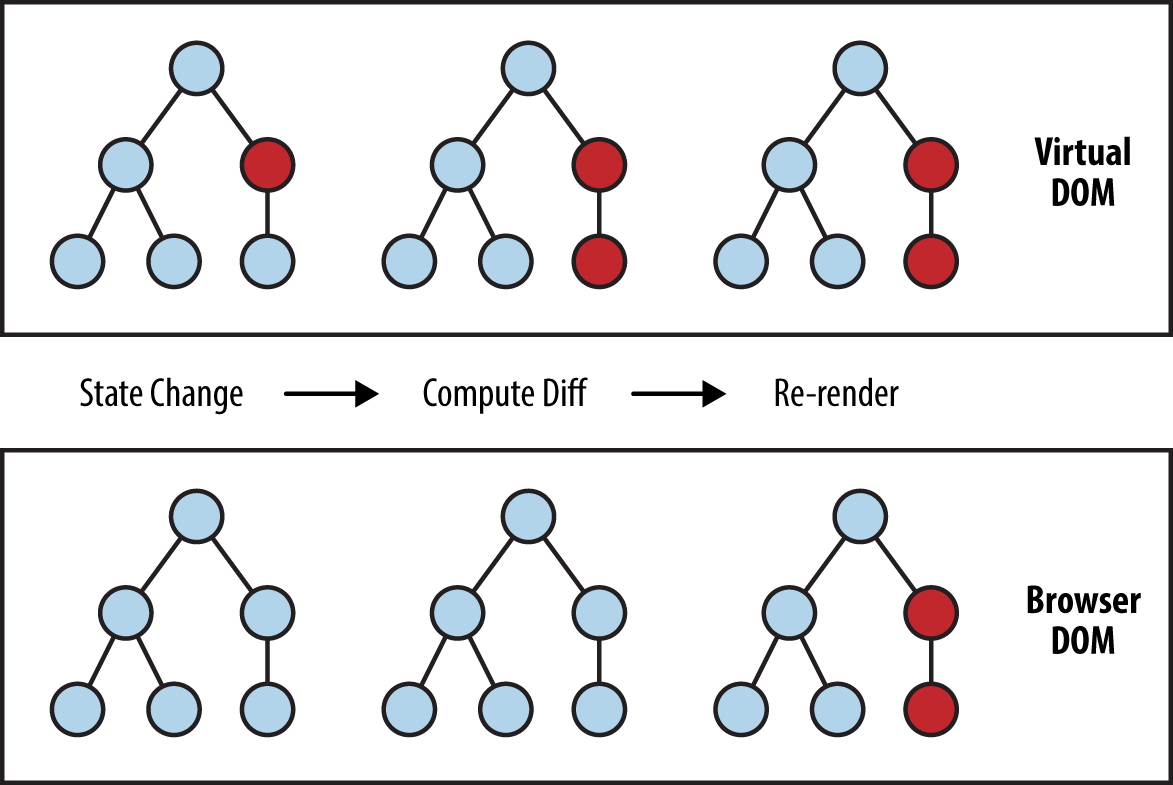
\includegraphics[width=0.8\textwidth]{images/cap4/react-virtual-dom.eps}
\caption{Funcionamiento del DOM virtual de React \cite{ReactVirtualDOM}}
\label{fig:Funcionamiento del DOM virtual de React}
\end{center}
\end{figure}

\subsection{El nuevo diseño por componentes}

Cada sección de la interfaz es realmente un componente independiente. Para modelar estas secciones 
adecuadamente se decidió importar los estilos de cada uno.

\bigskip
Sin embargo, esto se convirtió en un problema cualquier modificación de cáracter general requería
repetirlo a lo largo de los distintos ficheros. Es por eso, que se decidió utilizar la tecnología
Sass \cite{Sass}.

\bigskip
Esta tecnología se interpreta como CSS y añade entre múltiples características, el uso de variables. 
Con lo cual se pueden centralizar los estilos comunes como serían la fuente, el color.

\bigskip
Las características de React, permitieron hacer de esta una tarea mucho más sencilla de lo esperado en 
un principio.